\documentclass[handout]{beamer}
 
\usepackage[utf8]{inputenc}
\usepackage{mathtools}
\usepackage{tikz}
\usepackage{amsmath}

\usetheme{CambridgeUS}
% \useoutertheme{split}
\setbeamertemplate{title page}[default][colsep=-4bp,rounded=true]

% only inlcude the current secition in the header
\AtBeginSection{
    \begin{frame}
        \tableofcontents[sections=\value{section}, sectionstyle=show/show]
    \end{frame}
}

\usetikzlibrary{calc,shapes}
\usetikzlibrary{fit,positioning,decorations.pathreplacing,calligraphy}

\tikzstyle{key}=[circle, thin, minimum width=\ln, minimum height=\hn, draw=black, fill=white, inner sep=0cm, anchor=north]
\tikzstyle{fts}=[key,fill=gray!50,minimum width=0.8*\ln]
\tikzstyle{hash}=[key,rectangle, anchor=north]

\renewcommand{\ln}{6mm} % largeur de noeud
\newcommand{\hn}{6mm}    % hauteur de noeud
\renewcommand{\le}{5mm} % largeur de l'espace
\newcommand{\he}{8mm}   % hauteur de l'espace

\newcommand{\hasharrow}[2]{ \draw (H#2.north) -- ($(H#2.north)+(0,.5*\he)$) -- ($(H#1.south)+(0,-.5*\he)$) -> (H#1.south); }
\newcommand{\keyhasharrow}[2]{ \draw (K#2.north) -- ($(K#2.north)+(0,.5*\he)$) -- ($(H#1.south)+(0,-.5*\he)$) -> (H#1.south); }
\newcommand{\signarrow}[2]{ \draw (K#1.south) edge[dashed,->] (H#2.north); }


%Information to be included in the title page:
\title{Multi-Party Computation}
\author{Rohit Musti}
\institute{CUNY - Hunter College}
\date{\today}
 
\begin{document}
 
\frame{\titlepage}

\section{Overview}

\begin{frame}{Motivating Examples}
  \begin{itemize}
    \item \pause How can we compute on encrypted data?
    \item \pause How can Alice and Bob figure out who is wealthier without revealing their net worths?
    \item \pause How can Signal learn if any of your contacts are using signal without Signal learning anything?
    \item \pause How can two people check if their genome's share any characteristics without revealing any other information about their genomes?
    \item \pause How could we share ML training data without revealing our underlying datasets?
  \end{itemize} 
\end{frame}

\begin{frame}{Homework Example: Voting Problem}
  \begin{itemize}
    \item \pause Recall from HW 1, the challenge of computing the vote of the class
    \item \pause This protocol had some notable security flaws (two actors could collaborate and discover someone else's vote) (someone could lie about their vote)
    \item \pause However, it is a good example of multi-party computation as honest actors can collaborate to compute the collective vote
  \end{itemize}
\end{frame}

\begin{frame}{Warm Up}
  \begin{itemize}
    \item \pause Can we securely compute XOR?
    \item \pause Can we securely compute OR?
    \item \pause Can we securely compute AND?
  \end{itemize}
\end{frame}

\section{Oblivious Transfer}

\begin{frame}{Oblivious Transfer}
  \begin{itemize}
    \item \pause The most simple building block of multi-party computation
    \item \pause The idea is to establish a portocol where the sender has two messages \((m_0, m_1)\) and the receiver learns the details of one of the messages, but not the other, and the sender doesn't know which one the receiver learned
  \end{itemize}
\end{frame}

\begin{frame}{Oblivious Transfer: Random Oracles}
    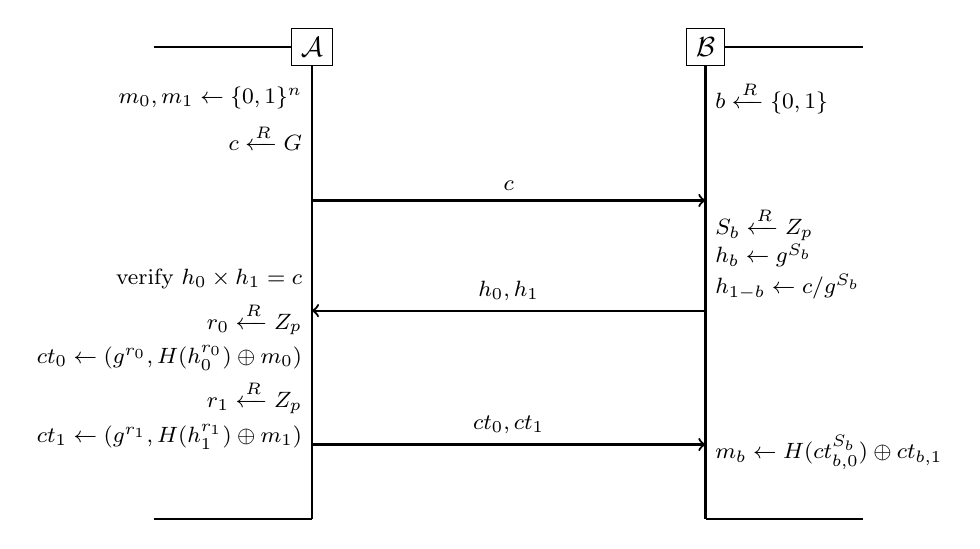
\begin{tikzpicture}
      \pause
        \node[draw] (Adversary) at (-3, 2) {\(\mathcal{A}\)}; 
        \draw[thick] (Adversary) -- ++(0, -6); 
        \draw[thick] (Adversary) -- ++(-2, 0);
        \draw[thick] (-3, -4) -- ++(-2, 0);

      \pause
        \node[draw] (Challenger) at (2,2) {\(\mathcal{B}\)}; 
        \draw[thick] (Challenger) -- ++(0, -6);
        \draw[thick] (Challenger) -- ++(2, 0);
        \draw[thick] (2, -4) -- ++(2, 0);

      \pause
        \node[draw=none,fill=none,anchor=west, font=\footnotesize] (bit) at ($(Challenger) + (0,-0.65)$) {\(b \xleftarrow[]{R} \{0, 1\}\)};
      \pause
        \node[draw=none,fill=none,anchor=east, font=\footnotesize] (choice0) at ($(Adversary) + (0,-.65)$) {\(m_0, m_1 \leftarrow \{0, 1\}^n\)};
      \pause
        \node[draw=none,fill=none,anchor=east, font=\footnotesize] (choice0) at ($(Adversary) + (0,-1.15)$) {\(c \xleftarrow[]{R} G\)};
      \pause
        \draw[->,thick] ($(Adversary)+(0,-1.95)$) -- ($(Challenger)+(0,-1.95)$) node [pos=0.5,above,font=\footnotesize] {\(c\)};
      \pause
        \node[draw=none,fill=none,anchor=west, font=\footnotesize] (bit) at ($(Challenger) + (0,-2.25)$) {\(S_b \xleftarrow[]{R} \mathbb{Z}_p\)};
      \pause
        \node[draw=none,fill=none,anchor=west, font=\footnotesize] (bit) at ($(Challenger) + (0,-2.65)$) {\(h_b \leftarrow g^{S_b}\)};
        \node[draw=none,fill=none,anchor=west, font=\footnotesize] (bit) at ($(Challenger) + (0,-3.05)$) {\(h_{1-b} \leftarrow c/g^{S_b}\)};
      \pause
        \draw[->,thick] ($(Challenger)+(0,-3.35)$) -- ($(Adversary)+(0,-3.35)$) node [pos=0.5,above,font=\footnotesize] {\(h_0,h_1 \)};
      \pause
        \node[draw=none,fill=none,anchor=east, font=\footnotesize] (choice0) at ($(Adversary) + (0,-2.95)$) {verify \(h_0 \times h_1 = c\)};
      \pause
        \node[draw=none,fill=none,anchor=east, font=\footnotesize] (choice0) at ($(Adversary) + (0,-3.45)$) {\(r_0 \xleftarrow[]{R} \mathbb{Z}_p\)};
        \node[draw=none,fill=none,anchor=east, font=\footnotesize] (choice0) at ($(Adversary) + (0,-3.95)$) {\(ct_0 \leftarrow (g^{r_0}, H(h_{0}^{r_0}) \oplus m_0) \)};
      \pause
        \node[draw=none,fill=none,anchor=east, font=\footnotesize] (choice0) at ($(Adversary) + (0,-4.45)$) {\(r_1 \xleftarrow[]{R} \mathbb{Z}_p\)};
        \node[draw=none,fill=none,anchor=east, font=\footnotesize] (choice0) at ($(Adversary) + (0,-4.95)$) {\(ct_1 \leftarrow (g^{r_1}, H(h_{1}^{r_1}) \oplus m_1) \)};
      \pause
        \draw[->,thick] ($(Adversary)+(0,-5.05)$) -- ($(Challenger)+(0,-5.05)$) node [pos=0.5,above,font=\footnotesize] {\(ct_0, ct_1\)};
      \pause
        \node[draw=none,fill=none,anchor=west, font=\footnotesize] (bit) at ($(Challenger) + (0,-5.15)$) {\(m_b \leftarrow H(ct_{b,0}^{S_b}) \oplus ct_{b,1}\)};
      \end{tikzpicture}
\end{frame}

\begin{frame}{Oblivious Transfer: No RO}
    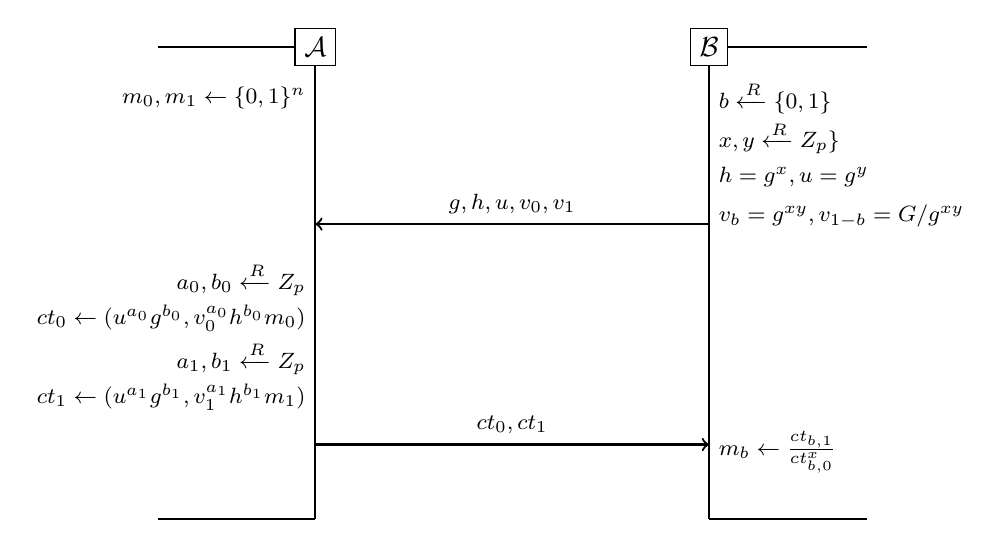
\begin{tikzpicture}
      \pause
        \node[draw] (Adversary) at (-3, 2) {\(\mathcal{A}\)}; 
        \draw[thick] (Adversary) -- ++(0, -6); 
        \draw[thick] (Adversary) -- ++(-2, 0);
        \draw[thick] (-3, -4) -- ++(-2, 0);

      \pause
        \node[draw] (Challenger) at (2,2) {\(\mathcal{B}\)}; 
        \draw[thick] (Challenger) -- ++(0, -6);
        \draw[thick] (Challenger) -- ++(2, 0);
        \draw[thick] (2, -4) -- ++(2, 0);

      \pause
        \node[draw=none,fill=none,anchor=west, font=\footnotesize] (bit) at ($(Challenger) + (0,-0.65)$) {\(b \xleftarrow[]{R} \{0, 1\}\)};
      \pause
        \node[draw=none,fill=none,anchor=west, font=\footnotesize] (bit) at ($(Challenger) + (0,-1.15)$) {\(x,y \xleftarrow[]{R} \mathbb{Z}_p\}\)};
      \pause
        \node[draw=none,fill=none,anchor=west, font=\footnotesize] (bit) at ($(Challenger) + (0,-1.65)$) {\(h = g^x, u = g^y\)};
      \pause
        \node[draw=none,fill=none,anchor=west, font=\footnotesize] (bit) at ($(Challenger) + (0,-2.15)$) {\(v_b = g^{xy}, v_{1-b} = \mathbb{G}/g^{xy}\)};
      \pause
        \node[draw=none,fill=none,anchor=east, font=\footnotesize] (choice0) at ($(Adversary) + (0,-.65)$) {\(m_0, m_1 \leftarrow \{0, 1\}^n\)};
      \pause
        \draw[->,thick] ($(Challenger)+(0,-2.25)$) -- ($(Adversary)+(0,-2.25)$) node [pos=0.5,above,font=\footnotesize] {\(g, h, u, v_0, v_1 \)};
      \pause
        \node[draw=none,fill=none,anchor=east, font=\footnotesize] (choice0) at ($(Adversary) + (0,-2.95)$) {\(a_0, b_0 \xleftarrow[]{R} \mathbb{Z}_p\)};
      \pause
        \node[draw=none,fill=none,anchor=east, font=\footnotesize] (choice0) at ($(Adversary) + (0,-3.45)$) {\(ct_0 \leftarrow (u^{a_0}g^{b_0}, v_0^{a_0}h^{b_0}m_0) \)};
      \pause
        \node[draw=none,fill=none,anchor=east, font=\footnotesize] (choice0) at ($(Adversary) + (0,-3.95)$) {\(a_1, b_1 \xleftarrow[]{R} \mathbb{Z}_p\)};
        \node[draw=none,fill=none,anchor=east, font=\footnotesize] (choice0) at ($(Adversary) + (0,-4.45)$) {\(ct_1 \leftarrow (u^{a_1}g^{b_1}, v_1^{a_1}h^{b_1}m_1) \)};
      \pause
        \draw[->,thick] ($(Adversary)+(0,-5.05)$) -- ($(Challenger)+(0,-5.05)$) node [pos=0.5,above,font=\footnotesize] {\(ct_0, ct_1\)};
      \pause
        \node[draw=none,fill=none,anchor=west, font=\footnotesize] (bit) at ($(Challenger) + (0,-5.15)$) {\(m_b \leftarrow \frac{ct_{b,1}}{ct_{b,0}^x}\)};
      \end{tikzpicture}
\end{frame}

\section{Shamir Secret Key Sharing}

\begin{frame}{Shamir Secret Sharing: Review}
  \begin{itemize}
    \item \pause Recall our discussion of Shamir Secret sharing during the public key encryption lecture
    \item \pause Essentially, it allowed us to share a secret with an arbitrary number of people and allow any subset of them to come together to unlock the secret \item \pause I got a little excited and put it there early, now we will discuss how to actually compute it!
  \end{itemize}
\end{frame}

\begin{frame}{Shamir Secret Sharing: Mechanism}
  \pause
  \[shares = [(-3, 0), (2, 5), (-1, -4)]\]
  \pause
  \begin{multline*}
  f(x) = 0 \times \frac{(x - 2)(x-(-1))}{(-3 - 2)(-3-(-1))} + 5 \times \frac{(x-(-3))(x - (-1))}{(2 - (-3))(2 - (-1))} + \\ -4 \times \frac{(x - (-3))(x - 2)}{(-1 -(-3))(-1 - 2)}
  \end{multline*}
  \pause
  \begin{multline*}
  f(0) = 0 \times \frac{(0 - 2)(0-(-1))}{(-3 - 2)(-3-(-1))} + 5 \times \frac{(0-(-3))(0 - (-1))}{(2 - (-3))(2 - (-1))} +\\ -4 \times \frac{(0 - (-3))(0 - 2)}{(-1 -(-3))(-1 - 2)}
  \end{multline*}
  \pause
  \[f(0) = -3\]
\end{frame}

\section{Computing on Secret Shared Data}

\begin{frame}{Computing on Secret Data}
  \begin{itemize}
    \item \pause Supposed Alice, Bob, and Charlie are friends and Charlie wants to know how many marbles Alice and Bob have!
    \item \pause Alice gives two random numbers to Charlie and Bob. \pause Bob gives two random numbers to Alice and Charlie
    \item \pause Alice computes \((a_{total} - s_{ac} - s_{ab}) + s_{ba}\)
    \item \pause Bob computes \((b_{total} - s_{bc} - s_{ba}) + s_{ab}\)
    \item \pause Charlie computes \(s_{ac}+ s_{bc}\)
    \item \pause They all share their results and independently compute \((a_{total} - s_{ac} - s_{ab}) + s_{ba} + (b_{total} - s_{bc} - s_{ba}) + s_{ab} + s_{ac}+ s_{bc}\)
  \end{itemize}
\end{frame}

\end{document}